\section{Preparation of q-sample}
\label{part4}

Given a discrete Bayesian network, it is possible to sample the underlying probability distribution using a quantum circuit. Indeed, this sampling method allows leveraging the computational advantages introduced by quantum algorithms, particularly through amplitude amplification discussed in the previous sections. \cite{borujeni2021quantum}

\subsection{Description}
The construction of the quantum circuit preparing a state vector representative of the Bayesian network, called a \textit{q-sample}, is done in three main steps:
\begin{itemize}
\item[1] Associate each variable of the Bayesian network with one or more qubits (depending on the number of values taken by the variable).
\item[2] Associate the probabilities (marginal or conditional) of each variable with the amplitudes of the component states of the corresponding qubits.
\item[3] Assimilate the amplitudes of the quantum states using (controlled) rotation gates, in a topological order of the graph $G$.
\end{itemize}
Initially, we will consider the binary case where the variables of the Bayesian network take only two values.
\\
Let $\mathcal{B} = (G,\mathcal{X})$ be a Bayesian network with $G=(V,E)$ a directed acyclic graph and $\mathcal{X}=(X_i)_{i\in[\![1,k]\!]}$ a family of random variables taking values in $\{0,1\}$ defined on $(\Omega, \mathcal{F}, \mathbb{P})$. We define the isomorphism:
\begin{align*}
    \Psi : \mathcal{X} &\longrightarrow \mathbb{C}^2\\
    X_i &\longmapsto |\psi_i\rangle
\end{align*}
which associates each variable of the Bayesian network with a state vector implemented by a qubit of the circuit. Thus, we represent the family $\mathcal{X}$ of random variables by a single state vector using the tensor product:
\[|\psi\rangle = \bigotimes_{i=1}^{k}|\psi_i\rangle \in (\mathbb{C}^2)^{\otimes k}\]
In practice, the vectors $|\psi_i\rangle$\footnotemark \ are initialized to $|0\rangle$ during their initialization in the circuit. We must then assign them the appropriate amplitudes to obtain the probabilities of the random variable upon measurement. In other words, for all $i\in[\![1,k]\!]$, we want to obtain:
\[|\psi_i\rangle = \alpha_i|0\rangle + \beta_i|1\rangle\]
with $|\alpha_i|^2 = \mathbb{P}(X_i=0)$ and $|\beta_i|^2 = \mathbb{P}(X_i=1)$.
\footnotetext{For simplicity, we will use the terms "qubits" and "state vectors" interchangeably and similarly the terms "quantum gates" and "unitary operators".}
\\
We distinguish two cases:
\begin{itemize}
\item Variables $X_i$ without parents in $G$: These are treated first. We apply a rotation gate $R_Y$ with an angle $\theta$ to assign the probabilities of a random variable to its representative qubit. The definition of $R_Y$ and the calculation of $\theta$ are explained in subsection \ref{simple_rotation_calc}.
\item Variables $X_i$ with parents in $G$: These are treated second in a topological order of the graph $G$. Moreover, several angles will need to be calculated for the different rotations conditioned by the values taken by the parents of $X_i$. Since the variables are binary, for $|Pa(X_i)|=m_i$, we have $2^{m_i}$ rotations to determine and apply to the vector $|\psi_i\rangle$. These rotations are implemented by controlled rotation gates whose angles depend on the conditional probabilities of $X_i$. Their calculation is detailed in subsection \ref{multi_rotation_calc}.
\end{itemize}

\subsection{Bloch Sphere}
\label{section_Bloch}

\begin{figure}
\centering
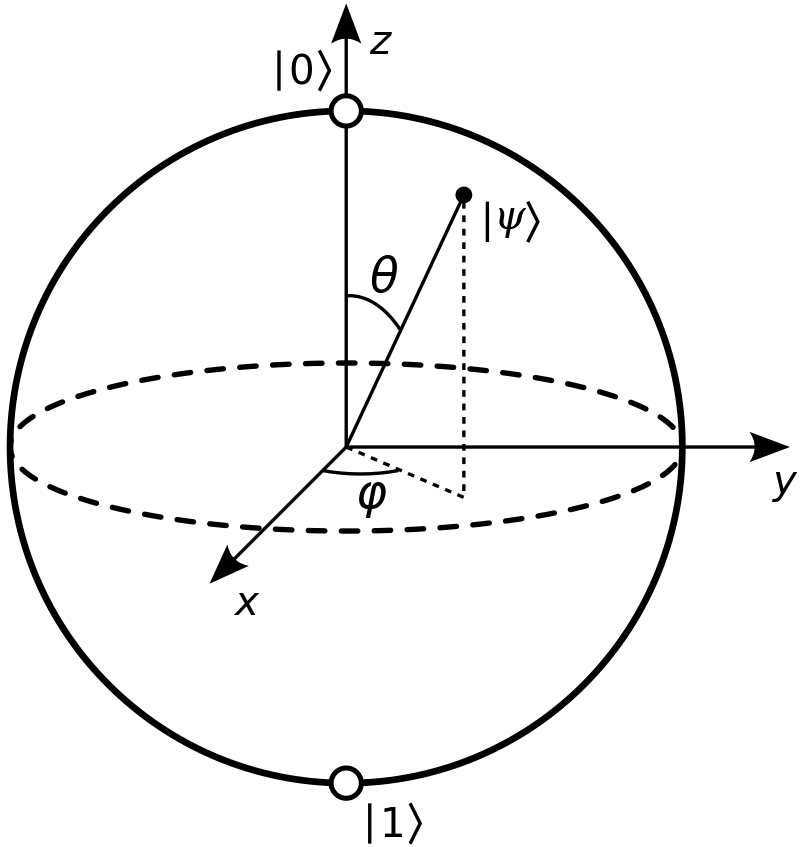
\includegraphics[scale=0.2]{Bloch_sphere}
\caption{The Bloch Sphere}
\label{fig:Bloch}
\end{figure}

First, let us define the Bloch sphere (Figure \ref{fig:Bloch}) which illustrates the transformations of quantum gates acting on a single qubit, including those of the $R_Y$ gate.
\\
Consider a state $|\psi \rangle =\alpha |0\rangle +\beta |1\rangle$ with amplitudes $\alpha ,\beta \in \mathbb{C}$ and $|\alpha|^{2}+|\beta |^{2}=1$. In polar coordinates, there exist $r_{\alpha}, r_{\beta} \in \mathbb{R}_+$ and $\phi_{\alpha}, \phi_{\beta} \in [0,2\pi[$ such that:
\[|\psi \rangle = r_{\alpha}e^{i\phi_{\alpha}}|0\rangle + r_{\beta}e^{i\phi_{\beta}} |1\rangle\]
\\
Since $|re^{i\phi}|^2 = re^{i\phi}re^{-i\phi} = r^2$, the probability of observing a qubit is entirely determined by the modulus of its amplitude. Thus, we define the equivalence relation $\sim$ on $\mathbb{C}^2$ by $\alpha \sim \beta \iff |\alpha|^2=|\beta|^2$. We then obtain:
\[|\psi \rangle \sim r_{\alpha}|0\rangle + r_{\beta}e^{i(\phi_{\beta}-\phi_{\alpha})} |1\rangle\]
Moreover, we notice that $r_{\alpha}^2+r_{\beta}^2=1$ so $r_{\alpha}, r_{\beta} \in [0,1]$. Consequently, the points $(r_{\alpha}, r_{\beta})$ belong to the first quadrant of the unit circle in $\mathbb{R}^2$. There is then a unique $\theta \in [0,\pi]$ such that $(r_{\alpha}, r_{\beta}) = (\mathrm{cos}(\theta/2),\mathrm{sin}(\theta/2))$. By setting $\phi = \phi_{\beta}-\phi_{\alpha} + 2n\pi$ with $n \in \mathbb{Z}$ so that $\phi \in [0,2\pi[$, we finally obtain:
\[|\psi \rangle \sim \mathrm{cos}(\theta/2)|0\rangle + \mathrm{sin}(\theta/2)e^{i\phi}|1\rangle\]
In this representation, we have:
\[(1,0,0) \cong \frac{|0\rangle+|1\rangle}{\sqrt{2}}, \ (0,1,0) \cong \frac{|0\rangle+i|1\rangle}{\sqrt{2}}, \ (0,0,1) \cong |0\rangle\]
and furthermore $|1\rangle \cong (0,0,-1)$.
\\
The remarkable point of this construction is that it allows us to study the qubits of $\mathbb{C}^2$ under the algebraic structure of $\mathbb{R}^3$ using spherical coordinates. Indeed, knowing that the graphical illustration of a complex number is done on a 2-dimensional plane, the Bloch sphere allows us to visualize 4-dimensional transformations using only 3 dimensions thanks to the previously defined equivalence relation.

\subsection{Rotation for Variables Without Parents}
\label{simple_rotation_calc}
Equipped with the Bloch sphere, the gate $R_Y(\theta)$ given in its matrix form by:
\begin{align*}
R_Y(\theta) = 
\begin{bmatrix}
\mathrm{cos}(\theta/2) & -\mathrm{sin}(\theta/2) \\
\mathrm{sin}(\theta/2) & \mathrm{cos}(\theta/2)
\end{bmatrix}
\end{align*}
performs a rotation around the Y-axis of the sphere by an angle of $\theta$ (hence the name $R_Y$). 
Knowing that a qubit is initialized to the state $|0\rangle$ at the beginning of the circuit, applying the $R_Y$ gate results in:
\[R_Y|0\rangle = \mathrm{cos}(\theta/2)|0\rangle+\mathrm{sin}(\theta/2)|1\rangle\]
The probabilities associated with the states $|0\rangle$ and $|1\rangle$ are therefore $\mathrm{cos}^2(\theta/2)$ and $\mathrm{sin}^2(\theta/2)$ respectively. Given a random variable $X_i$ without a parent in $G$, we want:
\[
\begin{cases}
\mathrm{cos}^2(\theta_{X_i}/2) = \mathbb{P}(X_i=0) \\
\mathrm{sin}^2(\theta_{X_i}/2) = \mathbb{P}(X_i=1)
\end{cases}
\]
Solving this system, we obtain:
\[
\theta_{X_i} = 
 \begin{cases}
 2\times\mathrm{arctan}\left(\sqrt{\frac{\displaystyle \mathbb{P}(X_i=1)}{\displaystyle \mathbb{P}(X_i=0)}}\right) & \mathrm{for} \ \mathbb{P}(X_i=0) \in \ ]0,1] \\
 \hfil \pi & \mathrm{for} \ \mathbb{P}(X_i=0)=0
 \end{cases}
\]
The value $\theta_{X_i}$ is therefore the appropriate rotation angle for the $R_Y$ gate to assign the probabilities of $X_i$ to the state vector $|0\rangle$. Since the $X_i$ have no parents in $G$, we can directly assign the calculated amplitudes to their representative qubit. This is why they are treated first.

\subsection{Rotation for Variables with Parents}
\label{multi_rotation_calc}
Similarly, for $X_i$ with parents in $G$, let $\Pi_{X_i}$ be the values taken by the parents of $X_i$, we have:
\[
\theta_{X_i,\Pi_{X_i}} = 
2\times\mathrm{arctan}\left(\sqrt{\frac{\displaystyle \mathbb{P}(X_i=1|Pa(X_i)=\Pi_{X_i})}{\displaystyle \mathbb{P}(X_i=0|Pa(X_i)=\Pi_{X_i})}}\right) 
\]
for $\mathbb{P}(X_i=0|Pa(X_i)=\Pi_{X_i}) \in \ ]0,1]$, and
$\theta_{X_i,\Pi_{X_i}} =  \pi$ when this probability is zero.
\\
Here $\theta_{X_i,\Pi_{X_i}}$ is the rotation angle to assign the conditional probabilities of $X_i$ to the values $\Pi_{X_i}$ taken by the parents of $X_i$. However, a direct application of the $R_Y$ gate is not suitable; it must also be conditioned on the qubits representing the variables of $Pa(X_i)$.
This brings us to controlled rotation gates.
\\
For $U$ a quantum gate, we define the controlled gate $CU$ acting on two qubits by the matrix:
\[CU =
\left[
\begin{array}{cccc}
    1 & 0 & 0 & 0 \\
    0 & 1 & 0 & 0 \\
    0 & 0 & \multicolumn{2}{c}{\smash{\raisebox{-.5\normalbaselineskip}{$U$}}} \\
    0 & 0 &  & 
\end{array}
\right]
\in \mathcal{M}_{4}(\mathbb{C})
\]
For a state vector $|\psi\rangle$, applying $CU$ to the tensor products on the left of $|\psi\rangle$ with the states $|0\rangle$ and $|1\rangle$ gives us:
\begin{align*}
CU (|0\rangle \otimes |\psi\rangle) =&\ |0\rangle \otimes |\psi\rangle \\
CU (|1\rangle \otimes |\psi\rangle) =&\ |1\rangle \otimes U|\psi\rangle 
\end{align*}
Here, the qubit $|x\rangle$ for $x\in\{0,1\}$ acts as a control of the gate $U$ on the target qubit $|\psi\rangle$. Indeed, we notice that $CU$ only applies the transformations of $U$ on $|\psi\rangle$ if $|x\rangle = |1\rangle$. For $|x\rangle = |0\rangle$, the qubit $|\psi\rangle$ remains unchanged. We also note that $CU$ does not perform any transformation on $|x\rangle$. 
\\
More generally, for $n\in\mathbb{N}^*$, the gate $C^nU$ acts on $n$ control qubits and 1 target qubit. Its matrix representation is given by the block matrix:
\[C^nU =
\left[
\begin{array}{cccc}
    I_2 & 0 & \hdots & 0 \\
    0 & \ddots & \ddots & \vdots \\
    \vdots & \ddots & I_2 & 0 \\
    0 & \hdots & 0 & U
\end{array}
\right]
\in \mathcal{M}_{2(n+1)}(\mathbb{C})
\]
with $0, \ I_2 \in \mathcal{M}_2(\mathbb{C})$ being the zero matrix and the identity matrix, respectively. 
\\
Given the state vector $|c_1 \hdots c_n\rangle \otimes |\psi\rangle$ with $n+1$ qubits, with $(|c_i\rangle)_{i\in[\![1,n]\!]}$ the control qubits and $|\psi\rangle$ the target qubit, we have:
\[C^nU(|c_1 \hdots c_n\rangle \otimes |\psi\rangle) = |c_1 \hdots c_n\rangle \otimes U|\psi\rangle \iff \forall i \in [\![1,n]\!], \ |c_i\rangle = |1\rangle \]
That is, the gate $C^nU$ performs the operation $U$ on $|\psi\rangle$ if and only if \textit{all} control qubits $|c_i\rangle$ are $|1\rangle$. 
In our case, a controlled rotation $C^{m_i}RY(\theta_{X_i, \Pi_{X_i}})$ acts on the vector $|c_1 \hdots c_{m_i}\rangle \otimes |\psi_i\rangle$, with $|\psi_i\rangle$ the representative qubit of the variable $X_i$, and $(|c_i\rangle)_{i\in[\![1,m_i]\!]}$ the representative qubits of the variables of $ Pa(X_i)$.
\\
Equipped with the gate $C^{m_i}RY(\theta_{X_i, \Pi_{X_i}})$, we are able to assign the corresponding amplitudes. However, knowing that the probabilities are conditioned by the values $\Pi_{X_i}$, and that the controlled gates only take effect when all control qubits are 1, we must first transform the qubits initialized to $|0\rangle$ into $|1\rangle$ before the passage of $C^{m_i}RY(\theta_{X_i, \Pi_{X_i}})$, and reconvert them to their initial state afterward.
Indeed, we want $C^{m_i}RY(\theta_{X_i, \Pi_{X_i}})$ to take effect whenever $Pa(X_i)=\Pi_{X_i}$, so we need to find a gate $B_{\Pi_{X_i}}$ acting on $|c_1 \hdots c_{m_i}\rangle$ such that:
\[
B_{\Pi_{X_i}}|c_1 \hdots c_{m_i}\rangle = |1\rangle^{\otimes m_i} \quad \mathrm{for} \quad (c_1,\hdots,c_{m_i}) = \Pi_{X_i}
\]
\\
For this, we use the $NOT$ gate given by:
\begin{align*}
NOT =
\left[
\begin{array}{cc}
    0 & 1 \\
    1 & 0
\end{array}
\right]
\in \mathcal{M}_{2}(\mathbb{C}) 
\end{align*}
where $NOT|0\rangle = |1\rangle$ and $NOT|1\rangle = |0\rangle$. 
The gate $B_{\Pi_{X_i}}$ is then expressed by the tensor product:
\[B_{\Pi_{X_i}} = \bigotimes_{k \in \Pi_{X_i}} NOT^{1-k} \]
Here, we used the fact that $\Pi_{X_i} \in \{0,1\}^{m_i}$ and that $NOT^0 = I_2$. 
\\
Finally, the operator describing the actions of all the gates resulting in the assignment of the amplitudes of a variable $X_i$ with parent values conditioned by $\Pi_{X_i}$ is given by: 
\[
\big(B_{\Pi_{X_i}} \!\! \otimes I_2 \big)
\big(C^{m_i}RY(\theta_{X_i, \Pi_{X_i}})\big)
\big(B_{\Pi_{X_i}} \!\! \otimes I_2 \big)
\]
This operation is then repeated for all possible combinations of the values $\Pi_{X_i}$ taken by the variables $Pa(X_i)$, so $2^{m_i}$ times as mentioned earlier.

\subsection{Representation of Discrete Variables with More Than Two Values}
\label{QBNgeneral}
For finite discrete random variables taking any number of values, these values must be binarized and several qubits used to represent a single variable. More precisely, for $X_i \in \mathcal{X}$, $N_i = |X_i(\Omega)|$ we use $n_i = \lceil \mathrm{log}_2(N_i) \rceil$ qubits. Revisiting the isomorphism defined in section \ref{part1}, we have $\Phi_i:[\![0,N_i-1]\!] \rightarrow (\mathbb{C}^2)^{\otimes n_i}$ which realizes this association.\footnote{To maintain the mathematical consistency of the presentation, the binary encoding of the morphisms $\Phi_i$ is done with the most significant bit on the right instead of the left. This "reversed" binarization is done by $\mathscr{B}'$. }

Thus, the state vector representing $X_i$ is given by:
\[|\psi_i\rangle = \sum_{x=0}^{N_i-1}\alpha_{i,x}|x\rangle\]
where $|x\rangle = \Phi_i(x)$ and $|\alpha_{i,x}|^2 = \mathbb{P}(X_i=x)$. 
\\
Rotations are more challenging in the general case because they involve multiple qubits. We must then proceed step by step, focusing on one qubit at a time. 
We will then explicitly write the state vector $|x\rangle \in (\mathbb{C}^2)^{\otimes n_i}$ with the tensor product of the qubits $|q_i\rangle \in \mathbb{C}^2$:
\[|q_1 \hdots q_{n_i}\rangle = |\mathscr{B}'(x,n_i)\rangle = |x\rangle \]
Initially, let $U_{X_i, [\![1,n_i]\!]}$ be the rotation gate that acts on $n_i$ qubits such that:
\[U_{X_i, [\![1,n_i]\!]}|0\rangle^{\otimes n_i} = |\psi_i\rangle\]
The principle is to find a decomposition of $U_{X_i, [\![1,n_i]\!]}$ in terms of $C^nRY$ and $NOT$. 
\\
For simplicity, we will omit the index $X_i$ from $U_{X_i, [\![1,n_i]\!]}$ indicating that it is the rotation concerning the variable $X_i$. The first step of decomposition is as follows:
\[U_{[\![1,n_i]\!]} = (\tilde{B}_{q_1} \cdot CU_{[\![2,n_i]\!],q_1=0} \cdot \tilde{B}_{q_1})(CU_{[\![2,n_i]\!],q_1=1})(RY(\theta_{q_1})\otimes I_2^{\otimes (n_i-1)})\]
Where $\tilde{B}_{q_1} = NOT \otimes I_2^{\otimes (n_i-1)}$ is the $NOT$ gate applied only to the first qubit $|q_1\rangle$, and $CU_{[\![2,n_i]\!],q_1=1}$ is the rotation gate acting on the qubits $(|q_i\rangle)_{i\in[\![2,n_i]\!]}$, conditioned with $|q_1\rangle=|1\rangle$ and controlled by the qubit $|q_1\rangle$. The gate $CU_{[\![2,n_i]\!],q_1=0}$ is defined analogously. 
\\
The idea here is to draw inspiration from the previous subsection concerning rotations for variables with parents to perform a binarization of the discrete variable.
\\
First, let us calculate $\theta_{q_1}$, the rotation angle allowing $R_Y$ to assign the amplitudes of the first qubit $|q_1\rangle$, with $q_1$ being the first element of $\mathscr{B}'(x,n_i)$. We define the indicator function:
\begin{align*}
    \mathbbm{1}_{q_1} : {\{0,1\}}^{n_i} &\longrightarrow \{0,1\} \\
    (q_1, \hdots ,q_{n_i}) &\longmapsto
 \begin{cases}
 1 \ \mathrm{if} \ q_1 = 1 \\
 0 \ \mathrm{if} \ q_1 = 0 
 \end{cases}
\end{align*}
The rotation value $\theta_{q_1}$ of the first qubit representing $X_i$ is then given by:
\begin{align*}
    \theta_{q_1} = 2\times\mathrm{arctan}\left[\sqrt{\frac{\displaystyle \mathbb{P}(\mathbbm{1}_{q_1}(\mathscr{B}'(X_i,n_i))=1)}{\displaystyle \mathbb{P}(\mathbbm{1}_{q_1}(\mathscr{B}'(X_i,n_i))=0)}}\right] \footnotemark
\end{align*}
\footnotetext{By abuse of notation, we can see this as $2\times\mathrm{arctan}\left[\sqrt{\frac{\displaystyle \mathbb{P}(q_1=1)}{\displaystyle \mathbb{P}(q_1=0)}}\right]$. }
Summing over $X_i(\Omega)$, we obtain:
\begin{align*}
    \mathbb{P}(\mathbbm{1}_{q_1}(\mathscr{B}'(X_i,n_i))=1) =&\ \sum_{x=0}^{N_i-1}\mathbb{P}(X_i=x)\mathbb{P}(\mathbbm{1}_{q_1}(\mathscr{B}'(X_i,n_i))=1|X_i=x) \\
    =&\ \sum_{x=0}^{N_i-1}\mathbb{P}(X_i=x)\mathbbm{1}_{q_1}(\mathscr{B}'(X_i,n_i)) \\
    =&\ \sum_{x=0}^{N_i-1}|\alpha_{i,x}|^2\mathbbm{1}_{q_1}(\mathscr{B}'(X_i,n_i))
\end{align*}
Finally, using the fact that the two events are complementary, we obtain: 
\begin{align*}
    \theta_{q_1} = 2\times\mathrm{arctan}\left[\sqrt{\frac{\displaystyle \sum_{x=0}^{N_i-1}|\alpha_{i,x}|^2\mathbbm{1}_{q_1}\left(\mathscr{B}'(x,n_i)\right)}{\displaystyle 1-\sum_{x=0}^{N_i-1}|\alpha_{i,x}|^2\mathbbm{1}_{q_1}\left(\mathscr{B}'(x,n_i)\right)}}\right]
\end{align*}
Once the rotation of the first qubit is established, we use the same process to decompose the gates $CU_{[\![2,n_i]\!],q_1=1}$ and $CU_{[\![2,n_i]\!],q_1=0}$. 
\\
In general, for $j\in[\![1,n_i-2]\!]$, the rotation gate $C^jU_{[\![j+1,n_i]\!], q=s}$ acting on the qubits $(|q_i\rangle)_{i\in[\![j+1,n_i]\!]}$ conditioned by the word\footnotemark \ $s \in \{0,1\}^j$ and controlled by the qubits representing $q=(q_i)_{i\in[\![1,j]\!]}$ is decomposed by the following recurrence formula:
\footnotetext{Here the term "word" is used in the context of formal language, particularly $s = s_1 \cdots s_j$ is a word of length $j$ in the alphabet $\{0,1\}$. We also use the notation $q$ to denote the $j$-tuple $(q_1,\hdots,q_j)$. Finally, $s \cdot 0$ is the word $s$ concatenated with the letter $0$.} 
\[
C^jU_{[\![j+1,n_i]\!], q=s} = U_0 \cdot U_1 \cdot [C^jRY(\theta_{q_{j+1}, q=s})\otimes I_2^{\otimes (n_i-1-j)}]
\]
with
\begin{align*}
U_0 =&\ C^j\tilde{B}_{q_{j+1}} \cdot C^{j+1}U_{[\![j+2,n_i]\!], (q\cdot q_{j+1})=(s \cdot 0)} \cdot  C^j\tilde{B}_{q_{j+1}}  \\
U_1 =&\ \ \qquad \qquad C^{j+1}U_{[\![j+2,n_i]\!], (q\cdot q_{j+1})=(s\cdot 1)}
\end{align*}
and 
$C^j\tilde{B}_{q_{j+1}} = C^jNOT \otimes I_2^{\otimes (n_i-1-j)}$. 
Here, $\theta_{q_{j+1}, q=s}$ is calculated with the indicator function:
\begin{align*}
    \mathbbm{1}_{q_{j+1}, q=s} : {\{0,1\}}^{n_i} &\longrightarrow \{0,1\} \\
    (q_1, \hdots ,q_{n_i}) &\longmapsto
 \begin{cases}
 1 \ \mathrm{if} \ q_{j+1} = 1 \ \mathrm{and} \ q=s\\
 0 \ \mathrm{otherwise}
 \end{cases}
\end{align*}
We have:
\begin{align*}
    \theta_{q_{j+1}, q=s} =&\ 2\times\mathrm{arctan}\left[\sqrt{\frac{\displaystyle \mathbb{P}(\mathbbm{1}_{q_{j+1}}(\mathscr{B}'(X_i,n_i))=1|\mathbbm{1}_{q=s}(\mathscr{B}'(X_i,n_i))=1)}{\displaystyle \mathbb{P}(\mathbbm{1}_{q_{j+1}}(\mathscr{B}'(X_i,n_i))=0|\mathbbm{1}_{q=s}(\mathscr{B}'(X_i,n_i))=1)}}\right] \\
    =&\ 2\times\mathrm{arctan}\left[\sqrt{\frac{\displaystyle \mathbb{P}(\mathbbm{1}_{q_{j+1}, q=s}(\mathscr{B}'(X_i,n_i))=1)}{\displaystyle \mathbb{P}(\mathbbm{1}_{q_{j+1}, q=s}(\mathscr{B}'(X_i,n_i))=0)}}\right] \\
    =&\ 2\times\mathrm{arctan}\left[\sqrt{\frac{\displaystyle \sum_{x=0}^{N_i-1}|\alpha_{i,x}|^2\mathbbm{1}_{q_{j+1}, q=s}\left(\mathscr{B}'(x,n_i)\right)}{\displaystyle 1-\sum_{x=0}^{N_i-1}|\alpha_{i,x}|^2\mathbbm{1}_{q_{j+1}, q=s}\left(\mathscr{B}'(x,n_i)\right)}}\right]
\end{align*}
For $N_i=|X_i(\Omega)|$ this construction uses $2^{\lceil \mathrm{log}_2(N_i) \rceil}-1$ $C^nRY$ gates and $2^{\lceil \mathrm{log}_2(N_i) \rceil}-2$ $C^nNOT$ gates.
The total number of quantum gates used is thus bounded by:
\[\sum_{\substack{X_i \in \mathcal{X} \\ N_i = |X_i(\Omega)|}}
\left[
2^{\lceil \mathrm{log}_2(N_i)\rceil+1} \prod_{\substack{X_j\in Pa(X_i) \\ N_j = |X_j(\Omega)|}}N_j 
\right] 
\]
In particular, for a binary Bayesian network with $k$ variables, let $m = \underset{X_i\in\mathcal{X}}{\mathrm{max}}(|Pa(X_i)|)$ be the maximum in-degree. The complexity calculated in terms of the number of quantum gates is $\mathcal{O}(k2^m)$.
